\documentclass[a4paper]{report}
\usepackage[utf8]{inputenc}
\usepackage{graphicx}
\usepackage{titlepic}
\usepackage{minted}
\usepackage{ltablex}
\usepackage{textcomp}
\usepackage{tabularx}
\usepackage{float}
\usepackage{layout}
\usepackage{xurl}
% \usepackage[a4paper, total={7in, 8in}]{geometry}

\urlstyle{same}

\graphicspath{{./images}}

\usepackage[english]{babel}
\usepackage{packages/sleek}
\usepackage{packages/sleek-title}
\usepackage{packages/sleek-theorems}
\usepackage{packages/sleek-listings}



%opening
\logo{ju}
\institute{University of Jordan}
\faculty{Faculty of Computer Science}
\title{Malware Analysis Report}
\author{Ward M. Zahran\\ID: 0213853}
\subtitle{An Analysis of the Ryuk Ransomware}

\begin{document}

\maketitle
\pagebreak

\tableofcontents
\pagebreak

\chapter{Summary} 
\label{chap:Summary}

\section{Executive Summary}

\subsection{Objective}
To analyse a sample detected by our SOC team and understand the damage caused by it.

\subsection{Key Findings}
\begin{enumerate}
    \item 
        The sample is a ransomeware from the RYUK family. 
    \item 
        The sample uses hard coded asymetric keys.
    \item 
        The sample has the ability to encrypt remote file shares connected to the victim.
    \item 
        The sample uses some level of obfuscation in order to hide information from analysts.
\end{enumerate}

\section{Introduction}
Purpose: Our SOC team has detected a malware sample of unknown origin and would like to have a report of its network activity and general behavior.
Scope: Understand its network activities and how it generally operates as well as find IoCs to disallow future incidents.
Background: Ryuk is a family of ransomeware that targets finacial sectors with the end goal of making money via a ransom.



\chapter{Static Analysis} % (fold)
\label{chap:Static Analysis}

% chapter Static Analysis (end)

\section{File Information}

\subsection{Malware Type and Family}
The sample is a ransomware of the Ryuk family.

\subsection{File Hashes}
The sample is a Windows 32 bit executable and has the following hashes:
\begin{enumerate}
    \item 
        SHA256: 23e95ba67603234352ff2864dc7fa54742f501e5922f01f8c182dbefc116f97f
    \item
        SHA1: 	915FD6FB4E20909025F876F3BB453EC52E21B7BE
    \item 
        MD5:    7364f6222ac58896e8920f32e4d30aac
\end{enumerate}

\subsection{File Size}
The sample is a single file with the size of 121.50 Kb. 

No packing was detected using PEinfo nor with Exeinfo.

The file has an entropy of 6.4 making the odds of it being packed or obfuscated unlikely.

The sample was compiled in 2021 making it rather old, that is if the debug stamp is to be trusted, see Figure~\ref{fig:compile_stamp}.

\begin{figure}[H]
    \begin{center}
        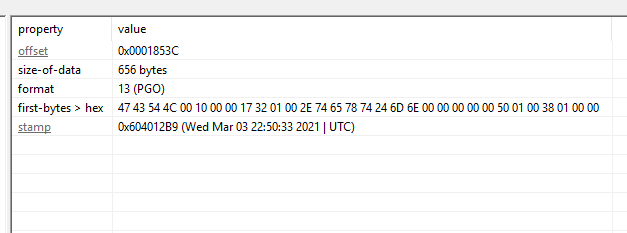
\includegraphics[width=0.95\textwidth]{compile_stamp}
    \end{center}
    \caption{Compiler stamp}\label{fig:compile_stamp}
\end{figure}


\section{Imports}
The sample uses the kernel32 and ws2\_32. The latter indicating network activity. See fig. 
Although looking at these imports are almost meaningless due to the fact that the executable actually imports functions that allow it to load libraries and execute them at runtime
instead of link time and thus the Imports won't fully appear, this will be covered more in-depth in the dynamic analysis part, see Figure~\ref{fig:libraries}.

\begin{figure}[H]
    \begin{center}
        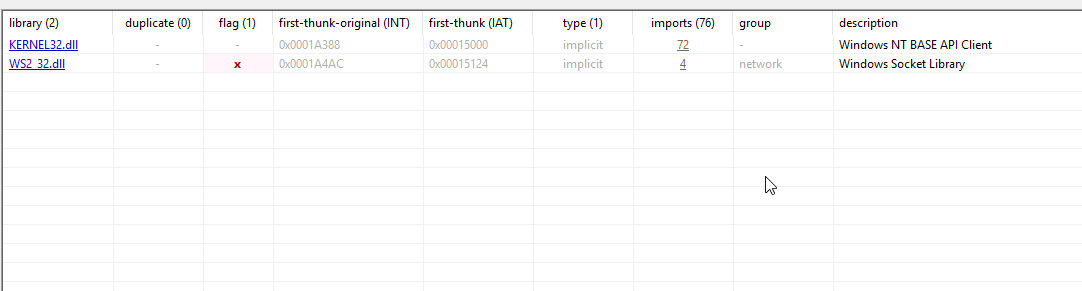
\includegraphics[width=0.95\textwidth]{libraries}
    \end{center}
    \caption{Used libraries}\label{fig:libraries}
\end{figure}

\section{Interesting Imports}
The functions related to runtime library loading can be seen in Figure~\ref{fig:dynamic_libraries}

\begin{figure}[H]
    \begin{center}
        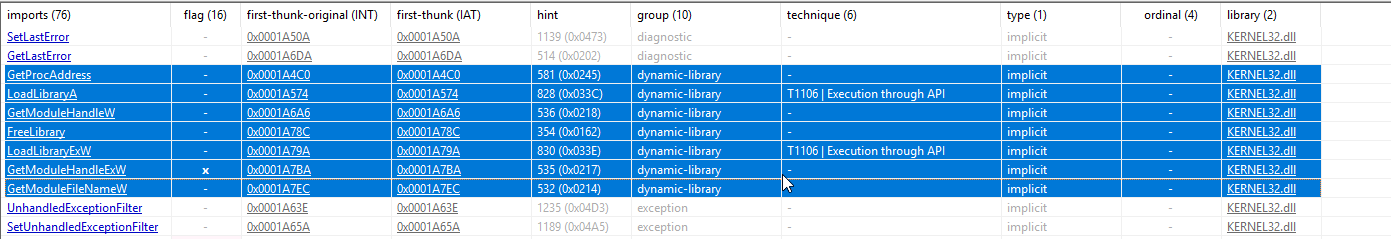
\includegraphics[width=0.95\textwidth]{dynamic_libraries}
    \end{center}
    \caption{Dynamic Library Related Imports}\label{fig:dynamic_libraries}
\end{figure}



\section{Strings Analysis}
String analysis using FLOSS resulted in many strings most interesting of which are:

Partial HTML string:
\begin{listing}[H]
    \caption{HTML found in the sample}
    \begin{minted}[linenos,frame=single]{HTML}
<html>
<body>
<style>p:hover{ background: black; color:white }</style>
<script>
</script>
<p onclick="info()" style="font-weight:bold;font-size:127\%;top:0;left:0;border: 1px sol
    \end{minted}
\end{listing}

And the following onion URL:

\url{http://rdmnobnbtxh5sm3iiczazaregkpyyub3gktwneeehx62tyot5bc4qhad.onion}

Other interesting strings:

password = '

torlink = '

RYUKTM

\section{Virtus Total Detection}
The sample triggered 59/71 engines on Virus Total, see Figure~\ref{fig:virustotal}.

\begin{figure}[H]
    \begin{center}
        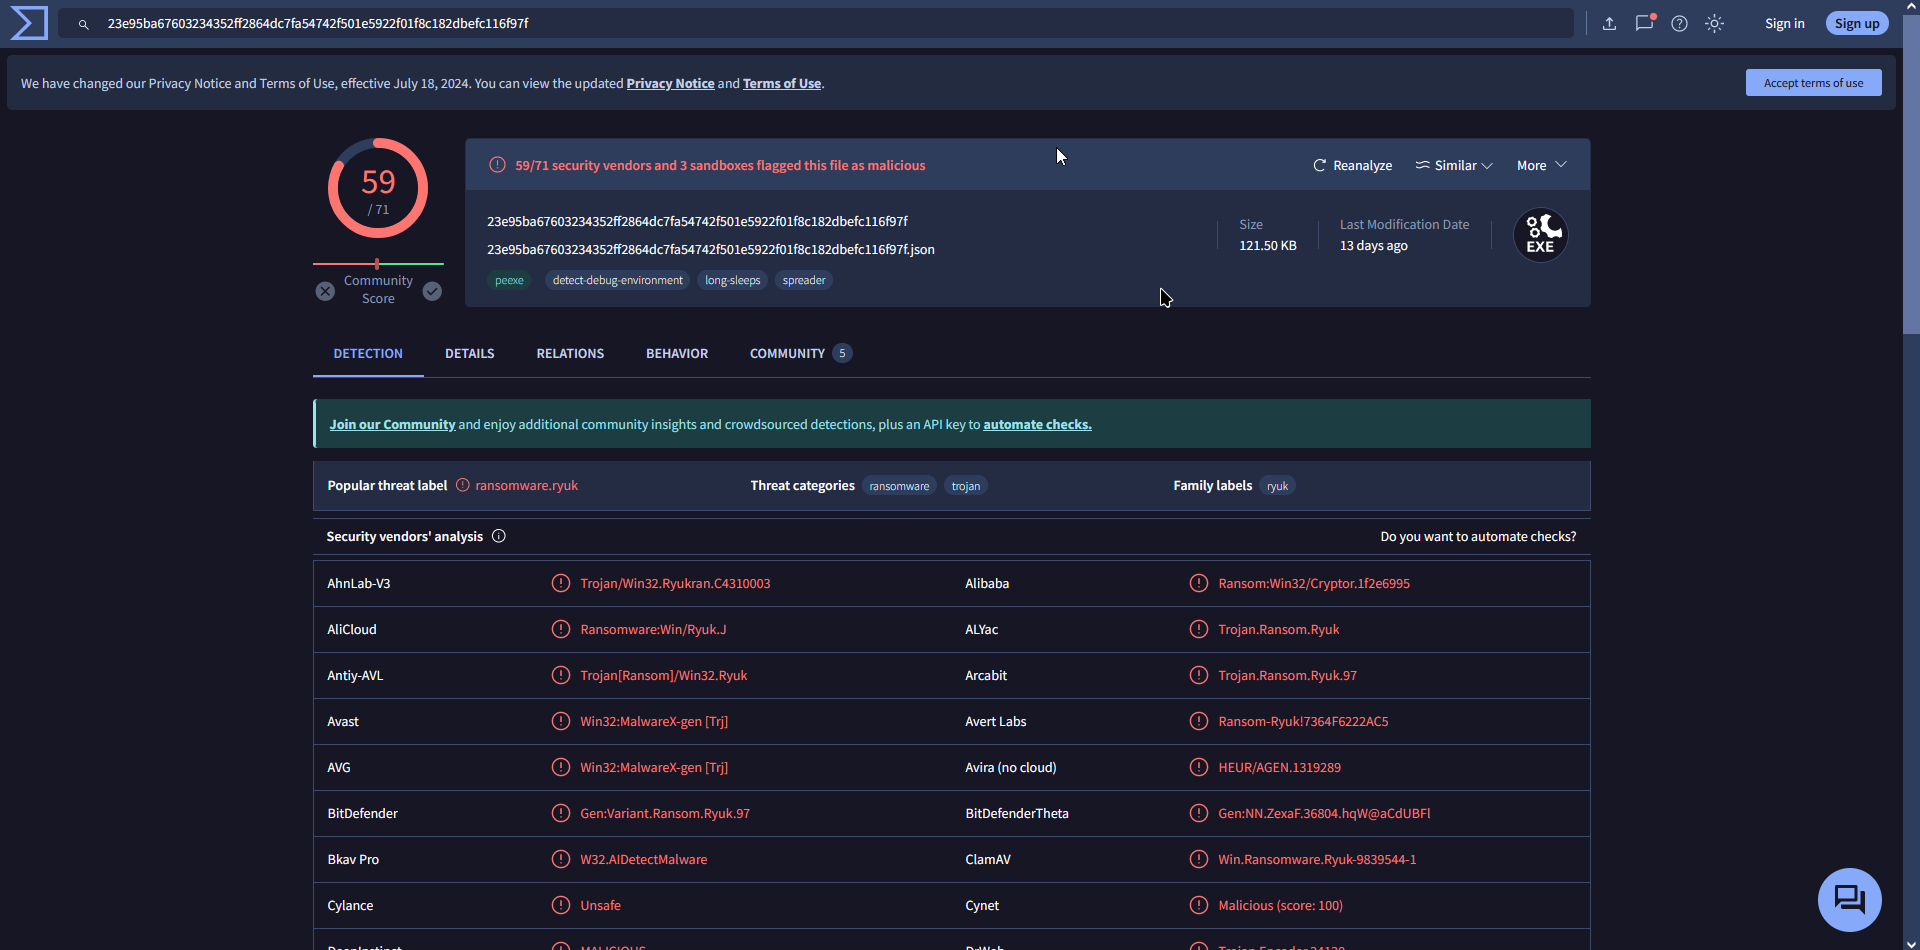
\includegraphics[width=0.95\textwidth]{virustotal}
    \end{center}
    \caption{Virus Total Scan}\label{fig:virustotal}
\end{figure}


\section{Code Analysis}
Code analysis is a pain due to my inexperience with Windows as well as the fact that some functions remain uresolved until runtime making static analysis using ghidra too much pain for what it is worth.

\section{Further Remarks}
The sample doesn't possess any ability to modify itself. see Figure~\ref{fig:no_self_modifying_code}.

\begin{figure}[H]
    \begin{center}
        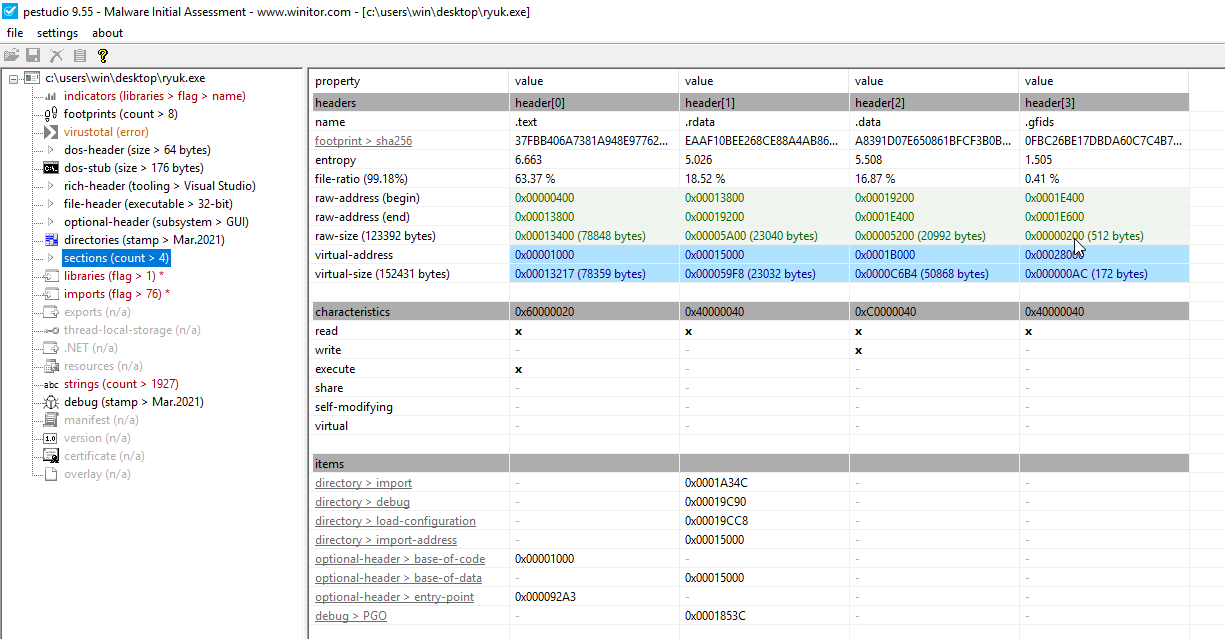
\includegraphics[width=0.95\textwidth]{no_self_modifying_code}
    \end{center}
    \caption{No self-modifying code abilities.}\label{fig:no_self_modifying_code}
\end{figure}


\chapter{Dynamic Analysis} 


\section{Execution}
Once the sample is run it begins to make hidden copies of itself with random names, each requesting to be ran as an adminstrator see Figure~\ref{fig:duplication}.
\begin{figure}
    \begin{center}
        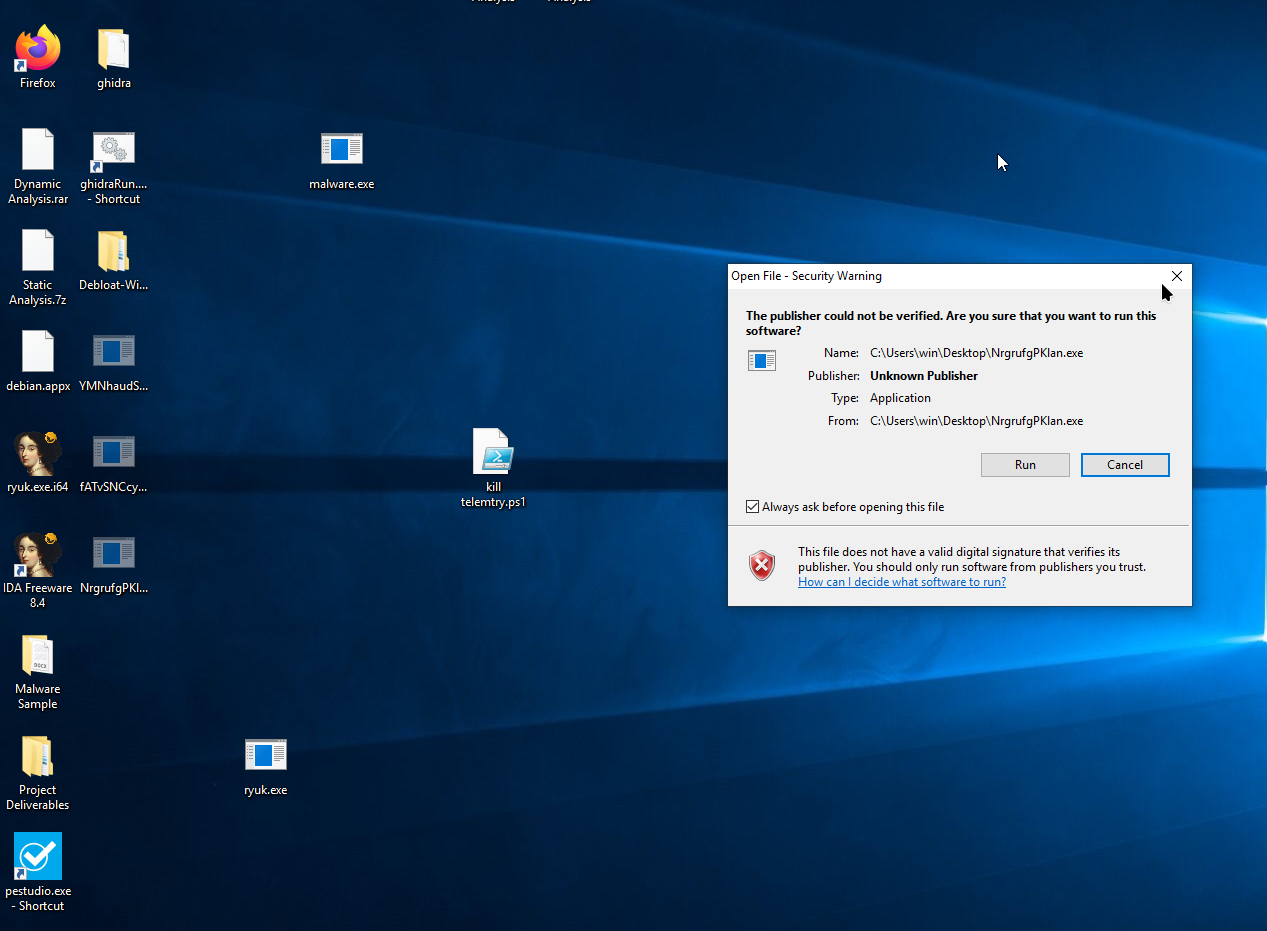
\includegraphics[width=0.95\textwidth]{duplication}
    \end{center}
    \caption{The sample copying itself 3 times.}\label{fig:duplication}
\end{figure}

After 3 copies are made the sample starts targeting anything except EXEs, DLLs and the Windows directory. Encrypted files gain the RYK extention. See Figure~\ref{fig:7zip_encrypted}.

\begin{figure}[H]
    \begin{center}
        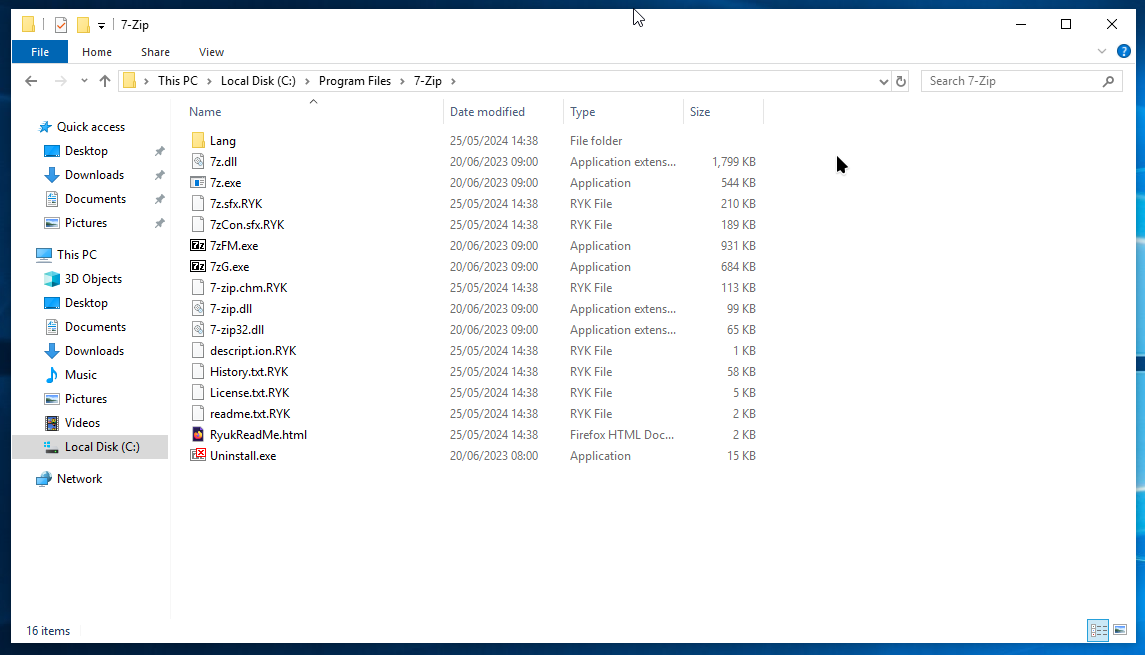
\includegraphics[width=0.95\textwidth]{7zip_encrypted}
    \end{center}
    \caption{Partially encrypted 7zip installation directory.}\label{fig:7zip_encrypted}
\end{figure}

Directories seem to be recursivly encrytped, in each directory an HTML file is generated showcasing how to decrypt files, see Figure~\ref{fig:html}.
\begin{figure}
    \begin{center}
        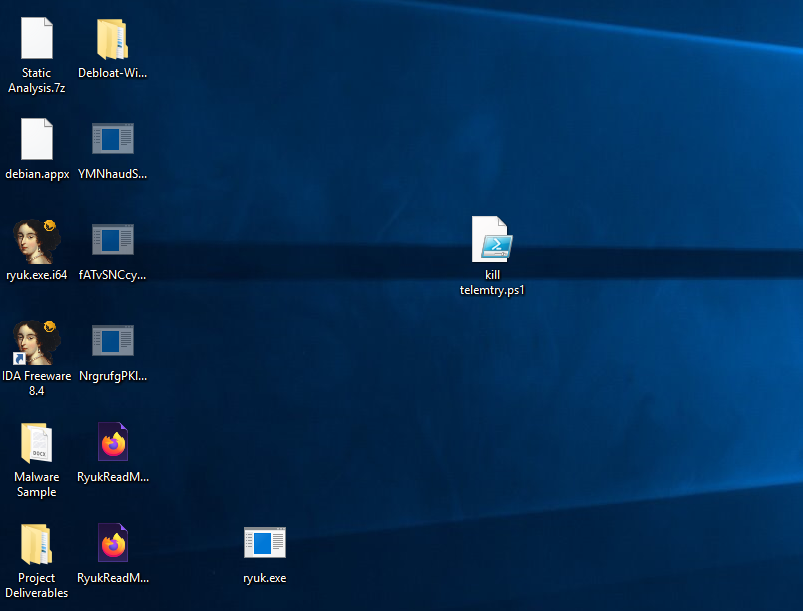
\includegraphics[width=0.95\textwidth]{html}
    \end{center}
    \caption{The HTML file containing decryption intsructions.}\label{fig:html}
\end{figure}

In the html file users are given a passwords and are directed to visit an onion address and submit the password in order to get decryption key. see Figure~\ref{fig:html_contents} and Figure~\ref{fig:onion_address}.

\begin{figure}[H]
    \begin{center}
        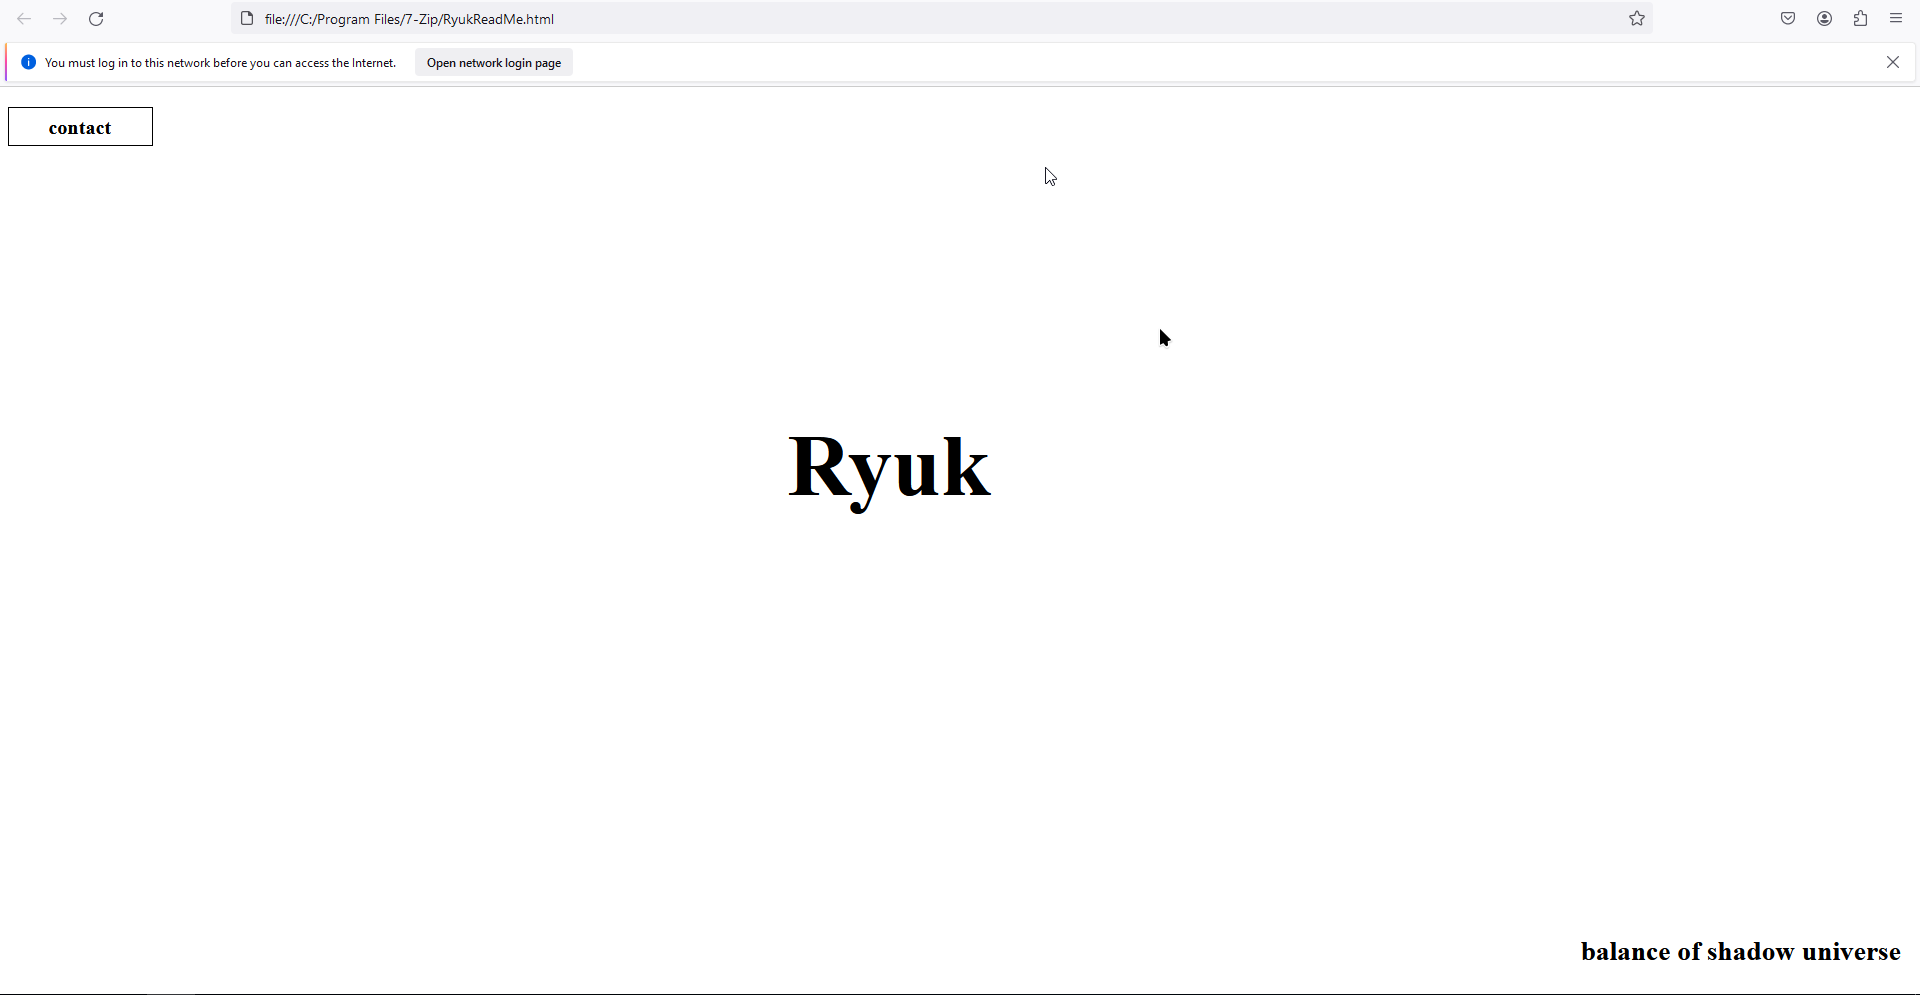
\includegraphics[width=0.95\textwidth]{html_contents}
    \end{center}
    \caption{The HTML file rendered in the browser}\label{fig:html_contents}
\end{figure}


\begin{figure}[H]
    \begin{center}
        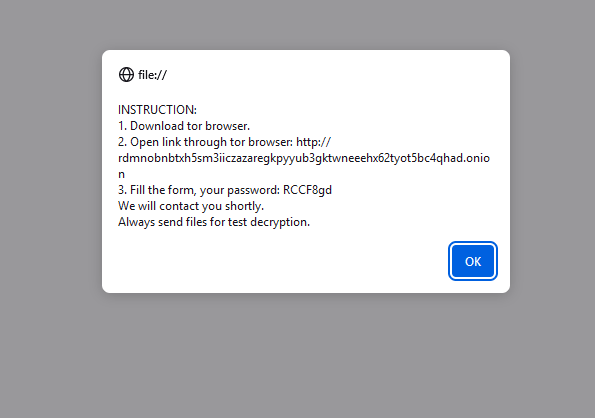
\includegraphics[width=0.95\textwidth]{onion_address}
    \end{center}
    \caption{Decryption instructions.}\label{fig:onion_address}
\end{figure}

The source code of the HTML file yeilds nothing of value. See Figure~\ref{fig:html_source}.

\begin{figure}[H]
    \begin{center}
        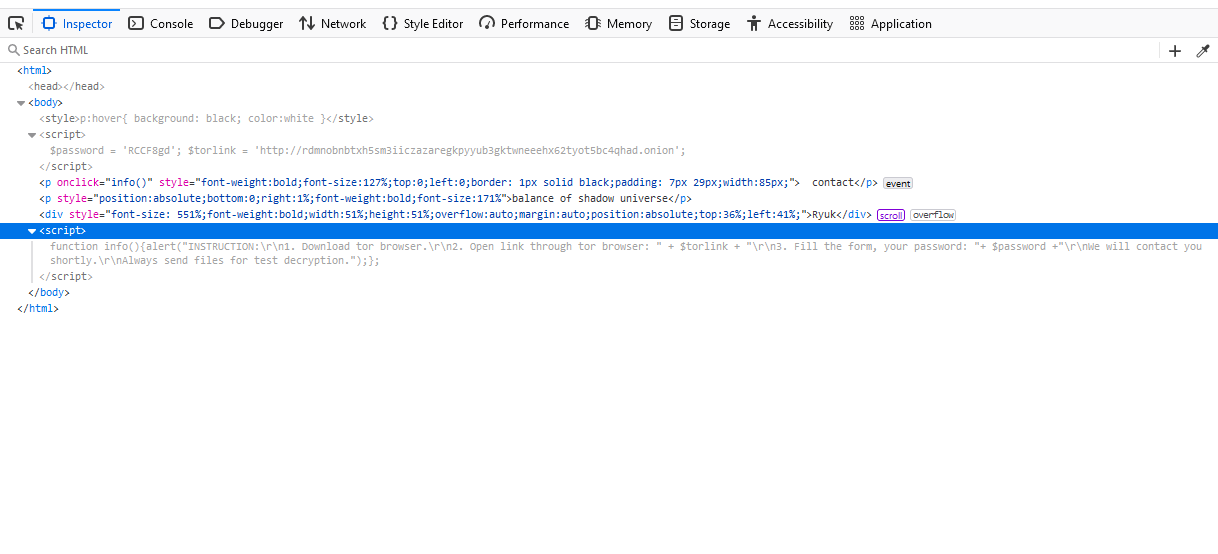
\includegraphics[width=0.95\textwidth]{html_source}
    \end{center}
    \caption{HTML source code.}\label{fig:html_source}
\end{figure}

The password seems to be executable dependent as running the same sample again even after reverting back to an old snapshot results in the same code,
meaning there is no need to transmit a decryption key over the network as the attacker can 
just have it hardcoded in the excutable instead via asymetric encryption. The network analysis seem but to confirm this.

As discussed earlier in the imports section, the sample uses functions to dynamically load libraries at runtime so we cannot get a full picture of the actual imports, that is unless we analyize each request to load 
a new DLL and then use that to get a comprehensive list, thankfully ProcMon provides us with the ability to do just that. See Figure~\ref{fig:full_imports} which showcases the full list of imported dlls for one of the copied samples.

\begin{figure}
    \begin{center}
        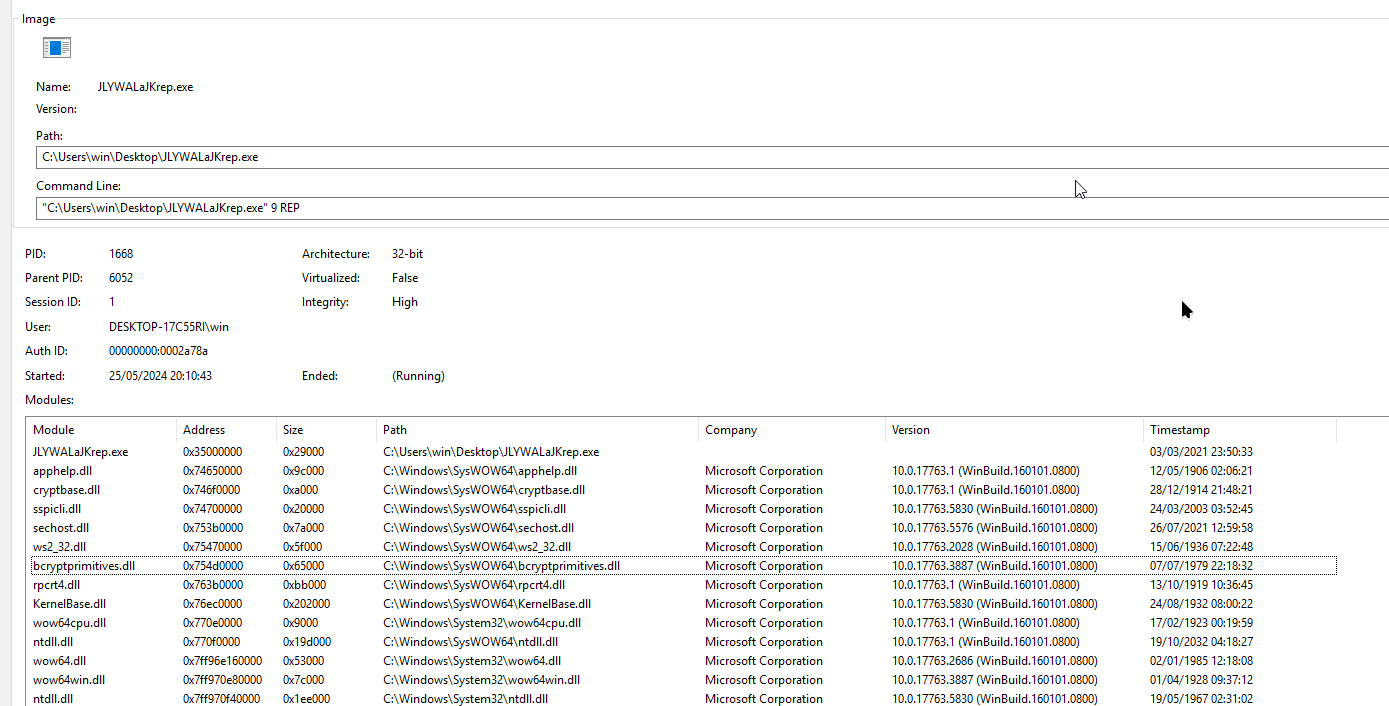
\includegraphics[width=0.95\textwidth]{full_imports}
    \end{center}
    \caption{A sample of the loaded DLLs.}\label{fig:full_imports}
\end{figure}

A full list of the loaded dlls can be found in \autoref{chap:Full List of Loaded DLLs}.
\section{Network Activity}
After starting, the sample starts spamming ARP requests to map out the network, once an active host is found it sends an ICMP ping request to the host. See Figure~\ref{fig:arp_request_spam}.
\begin{figure}[H]
    \begin{center}
        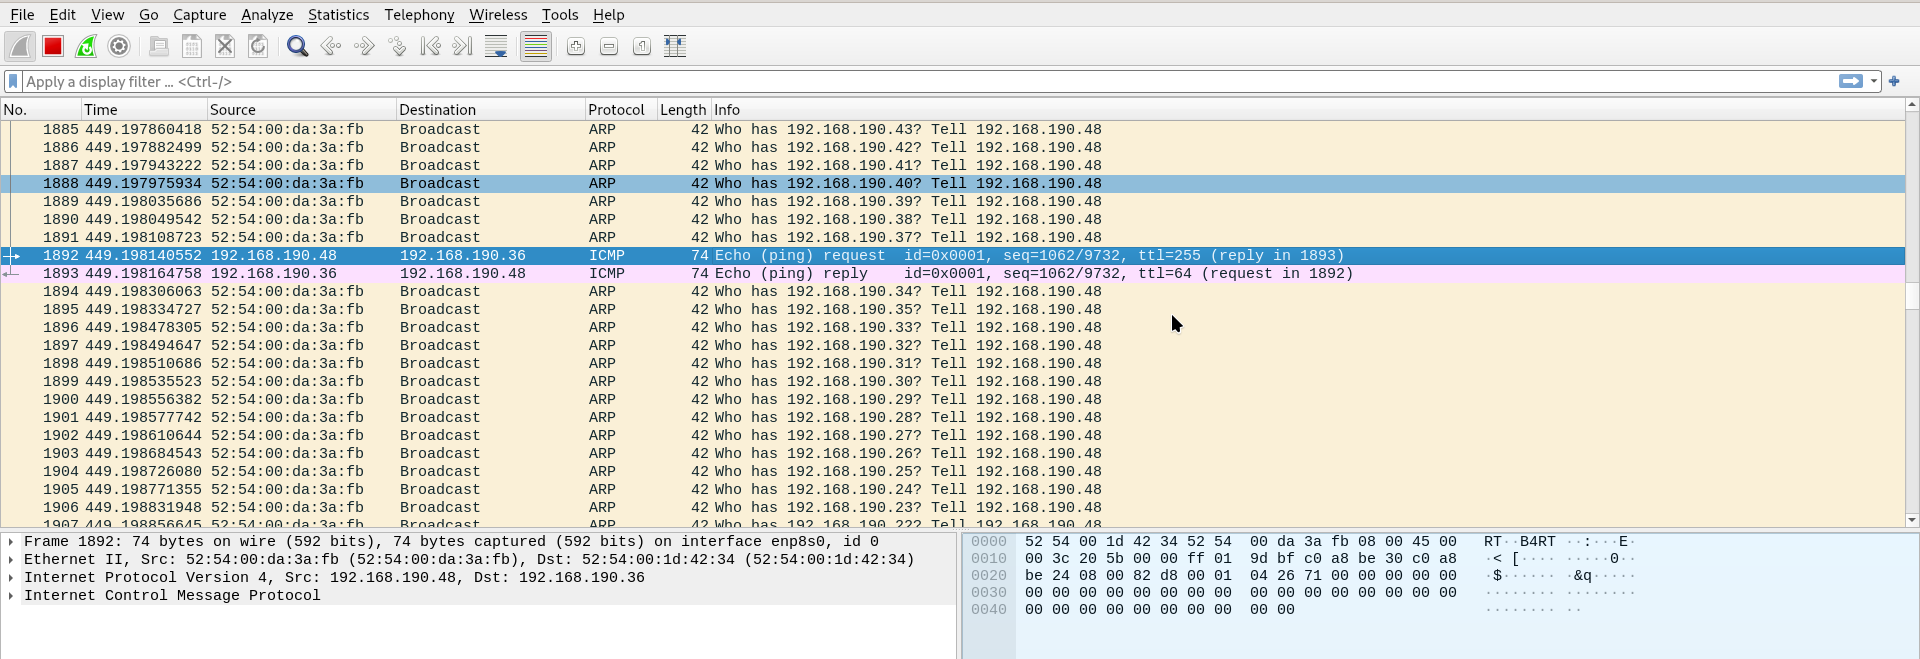
\includegraphics[width=0.95\textwidth]{arp_request_spam}
    \end{center}
    \caption{The sample mapping the network.}\label{fig:arp_request_spam}
\end{figure}

Only the initial process encrypts the local disk while all the other processes scan the network for any file shares and then try to encrypt them. See Figure~\ref{fig:network_encryption}.

\begin{figure}[H]
    \begin{center}
        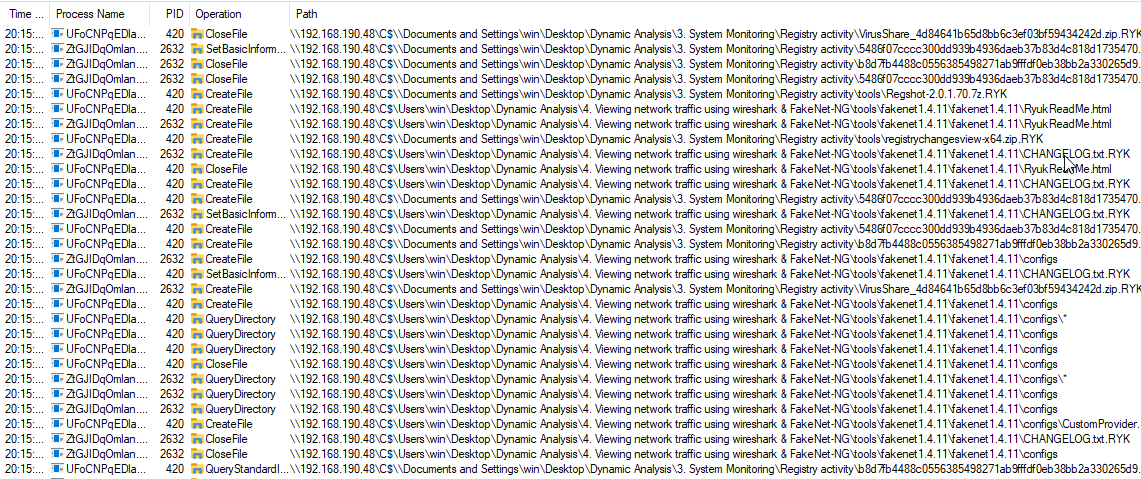
\includegraphics[width=0.95\textwidth]{network_encryption}
    \end{center}
    \caption{The sample attempting to encrypt the files over the network.}\label{fig:network_encryption}
\end{figure}

\section{File System Change}
Since the sample is a ransomeware it goes through each file opens it and then encrypts it and closes it. See Figure~\ref{fig:local_disk_encryption}.
\begin{figure}[H]
    \begin{center}
        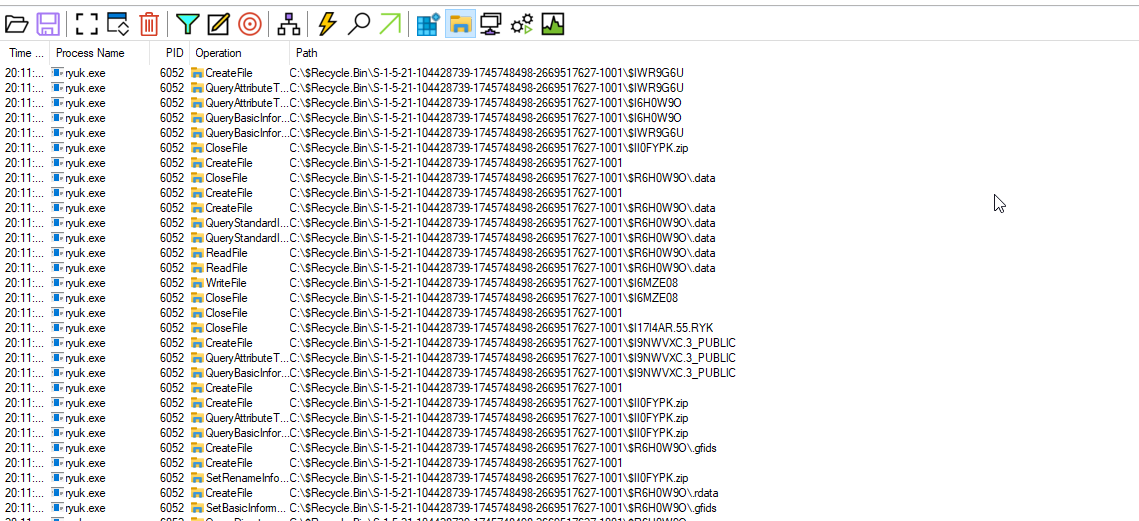
\includegraphics[width=0.95\textwidth]{local_disk_encryption}
    \end{center}
    \caption{The sample encrypting the local disk.}\label{fig:local_disk_encryption}
\end{figure}

The sample doesn't seem to have any persistance except for putting an html file in the user's startup folder in order to showcase the ransomware notice on boot.
\begin{figure}[H]
    \begin{center}
        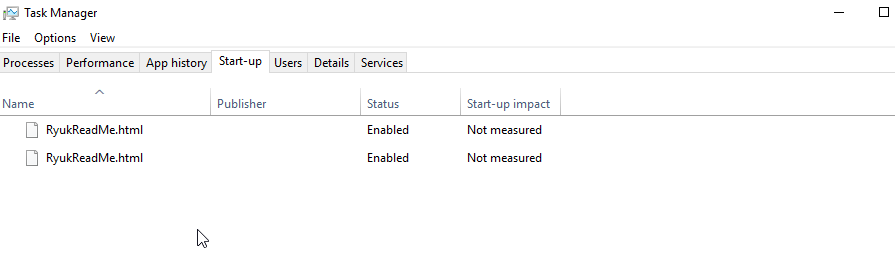
\includegraphics[width=0.95\textwidth]{startup}
    \end{center}
    \caption{The contents of the users startup directory after infection.}\label{fig:startup}
\end{figure}

As the contents of the Windows directory don't get encrypted we can abuse that fact by saving monitoring data into it.

\section{Registry Changes}
Only the initial launch of the sample results in any type of registery editing, all the copies only query the registry and to my very untrained eyes I didn't notice anything suspicious. See fig for all the keys modified
or created by the sample. See Figure~\ref{fig:registry_new_keys}
\begin{figure}[H]
    \begin{center}
        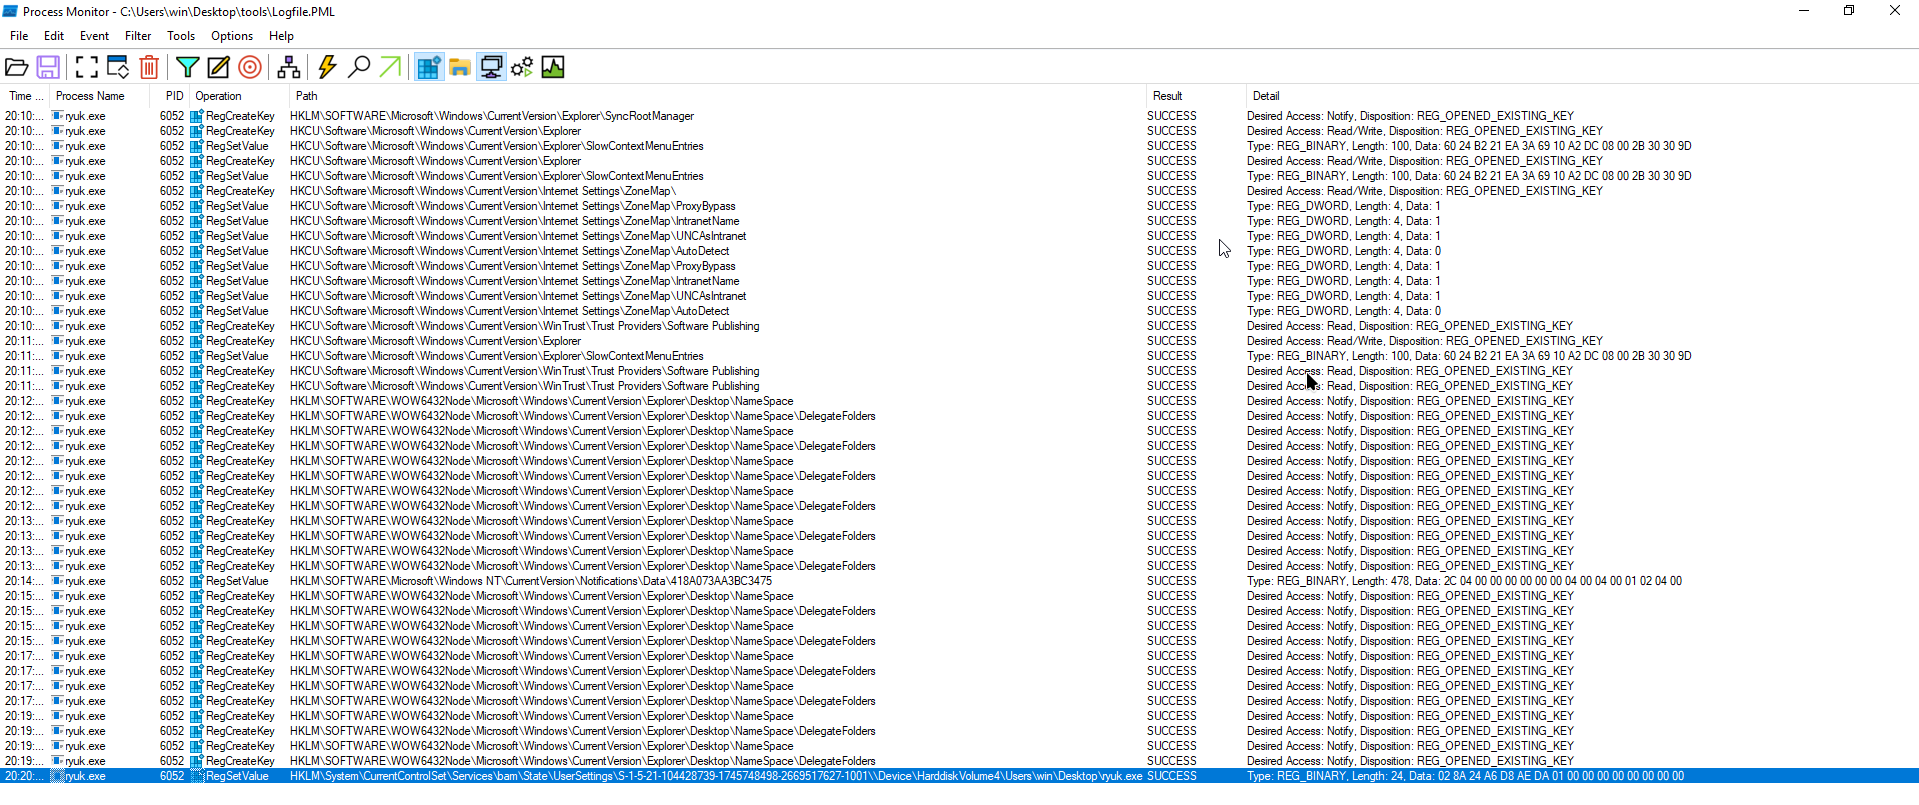
\includegraphics[width=0.95\textwidth]{registry_new_keys}
    \end{center}
    \caption{Modifications in the Windows registry.}\label{fig:registry_new_keys}
\end{figure}
In fact a comparision between Autoruns files from before and after running
the sample show zero differences, see Figure~\ref{fig:no_persistence_autorun}. Suffice to say the sample has no persistance other than the afformentioned HTML file.

\begin{figure}[H]
    \begin{center}
        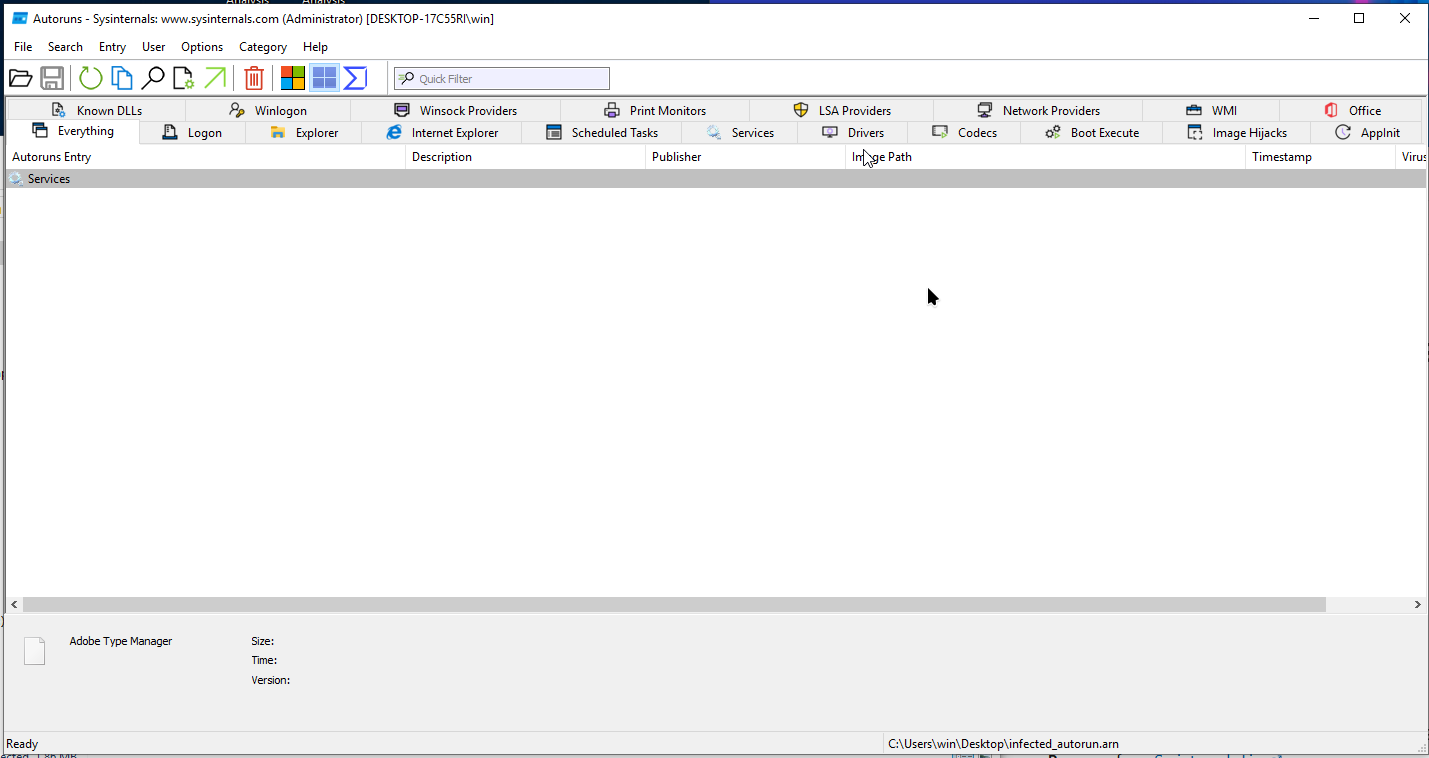
\includegraphics[width=0.95\textwidth]{no_persistence_autorun}
    \end{center}
    \caption{Autorun's compare feature showing no difference between autorunning apps before and after infection.}\label{fig:no_persistence_autorun}
\end{figure}



\chapter{IoC} % (fold)
\label{chap:IoC}

% chapter IoC (end)

\section{File Hashes}
\begin{enumerate}
    \item 
        SHA256: 23e95ba67603234352ff2864dc7fa54742f501e5922f01f8c182dbefc116f97f
    \item
        SHA1: 	915FD6FB4E20909025F876F3BB453EC52E21B7BE
    \item 
        MD5:    7364f6222ac58896e8920f32e4d30aac
\end{enumerate}
\section{IP Addresses}
None.
\section{Domain Names}
\url{http://rdmnobnbtxh5sm3iiczazaregkpyyub3gktwneeehx62tyot5bc4qhad.onion}
\section{Registry Keys}
None.


\chapter{Conclusion} % (fold)
\label{chap:Conclusion}

\section{Impact}
The sample has the ability to irrecoverly encrypt important documents from the victim PC and the network as a 
whole.
\section{Recommendations}
\begin{enumerate}
    \item 
        Contacting anti-virus vendors about the sample in order to add the sample to their databases.
    \item 
        Restoring from the newest available backup. 
    \item 
        Adding new rules to detect other similiar samples via the RYUK string within the binray.
\end{enumerate}

\appendix
\chapter{Full List of Loaded DLLs} % (fold)
\label{chap:Full List of Loaded DLLs}

\begin{enumerate}
    \item
        WinTypes.dll
    \item
        WinTypes.dll
    \item
        ryuk.exe (name of the executable itself)
    \item
        AppResolver.dll
    \item
        userenv.dll
    \item
        BCP47Langs.dll
    \item
        AppResolver.dll
    \item
        cldapi.dll
    \item
        WinTypes.dll
    \item
        CoreUIComponents.dll
    \item
        CoreMessaging.dll
    \item
        TextInputFramework.dll
    \item
        sppc.dll
    \item
        WindowsCodecs.dll
    \item
        dwmapi.dll
    \item
        comctl32.dll
    \item
        rsaenh.dll
    \item
        shdocvw.dll
    \item
        BCP47Langs.dll
    \item
        msvcp110\_win.dll
    \item
        policymanager.dll
    \item
        userenv.dll
    \item
        fltLib.dll
    \item
        virtdisk.dll
    \item
        srvcli.dll
    \item
        netutils.dll
    \item
        iertutil.dll
    \item
        urlmon.dll
    \item
        edputil.dll
    \item
        slc.dll
    \item
        smartscreenps.dll
    \item
        propsys.dll
    \item
        uxtheme.dll
    \item
        ntmarta.dll
    \item
        IPHLPAPI.DLL
    \item
        mpr.dll
    \item
        apphelp.dll
    \item
        cryptbase.dll
    \item
        msvcp\_win.dll
    \item
        powrprof.dll
    \item
        windows.storage.dll
    \item
        imagehlp.dll
    \item
        cfgmgr32.dll
    \item
        gdi32full.dll
    \item
        msasn1.dll
    \item
        imm32.dll
    \item
        ucrtbase.dll
    \item
        sechost.dll
    \item
        gdi32.dll
    \item
        ws2\_32.dll
    \item
        bcryptprimitives.dll
    \item
        profapi.dll
    \item
        msctf.dll
    \item
        shell32.dll
    \item
        clbcatq.dll
    \item
        wintrust.dll
    \item
        bcrypt.dll
    \item
        user32.dll
    \item
        advapi32.dll
    \item
        ole32.dll
    \item
        cryptsp.dll
    \item
        rpcrt4.dll
    \item
        oleaut32.dll
    \item
        crypt32.dll
    \item
        win32u.dll
    \item
        combase.dll
    \item
        SHCore.dll
    \item
        shlwapi.dll
    \item
        KernelBase.dll
    \item
        kernel.appcore.dll
    \item
        wow64cpu.dll
    \item
        ntdll.dll
    \item
        wow64.dll
    \item
        wow64win.dll
    \item
        ntdll.dll
\end{enumerate}

\listoffigures

% chapter List of figures (end)

\end{document}
